
\chapter*{Document of permissions}

On the following pages, I document the permissions for the use of all external materials in my dissertation. This includes:
\begin{itemize}
	\item The permission for using the Solar Wind Structures (SWS) list.
	\item The reprint permission for the article from Astronomy and Astrophysics (A\&A).
	\item A list of all 82 figures with their credits and permissions. I created 44 figures myself and display 38 figures from other sources. The figure permissions are backed either by my email correspondence, the RightsLink request result, or the obtained permission/license documents. NASA and NOAA content generally are not copyrighted\footnote{NASA Media Usage Guidelines website: \url{https://www.nasa.gov/multimedia/guidelines/}}\,\footnote{NOAA Copyright Information: \url{https://sos.noaa.gov/copyright-information}}.
	\end{itemize}

\vspace{2cm}

\noindent SWS list permission -- see the following email correspondence.
\lstinputlisting{permissions/Richardson_SWS_List_raw.txt}

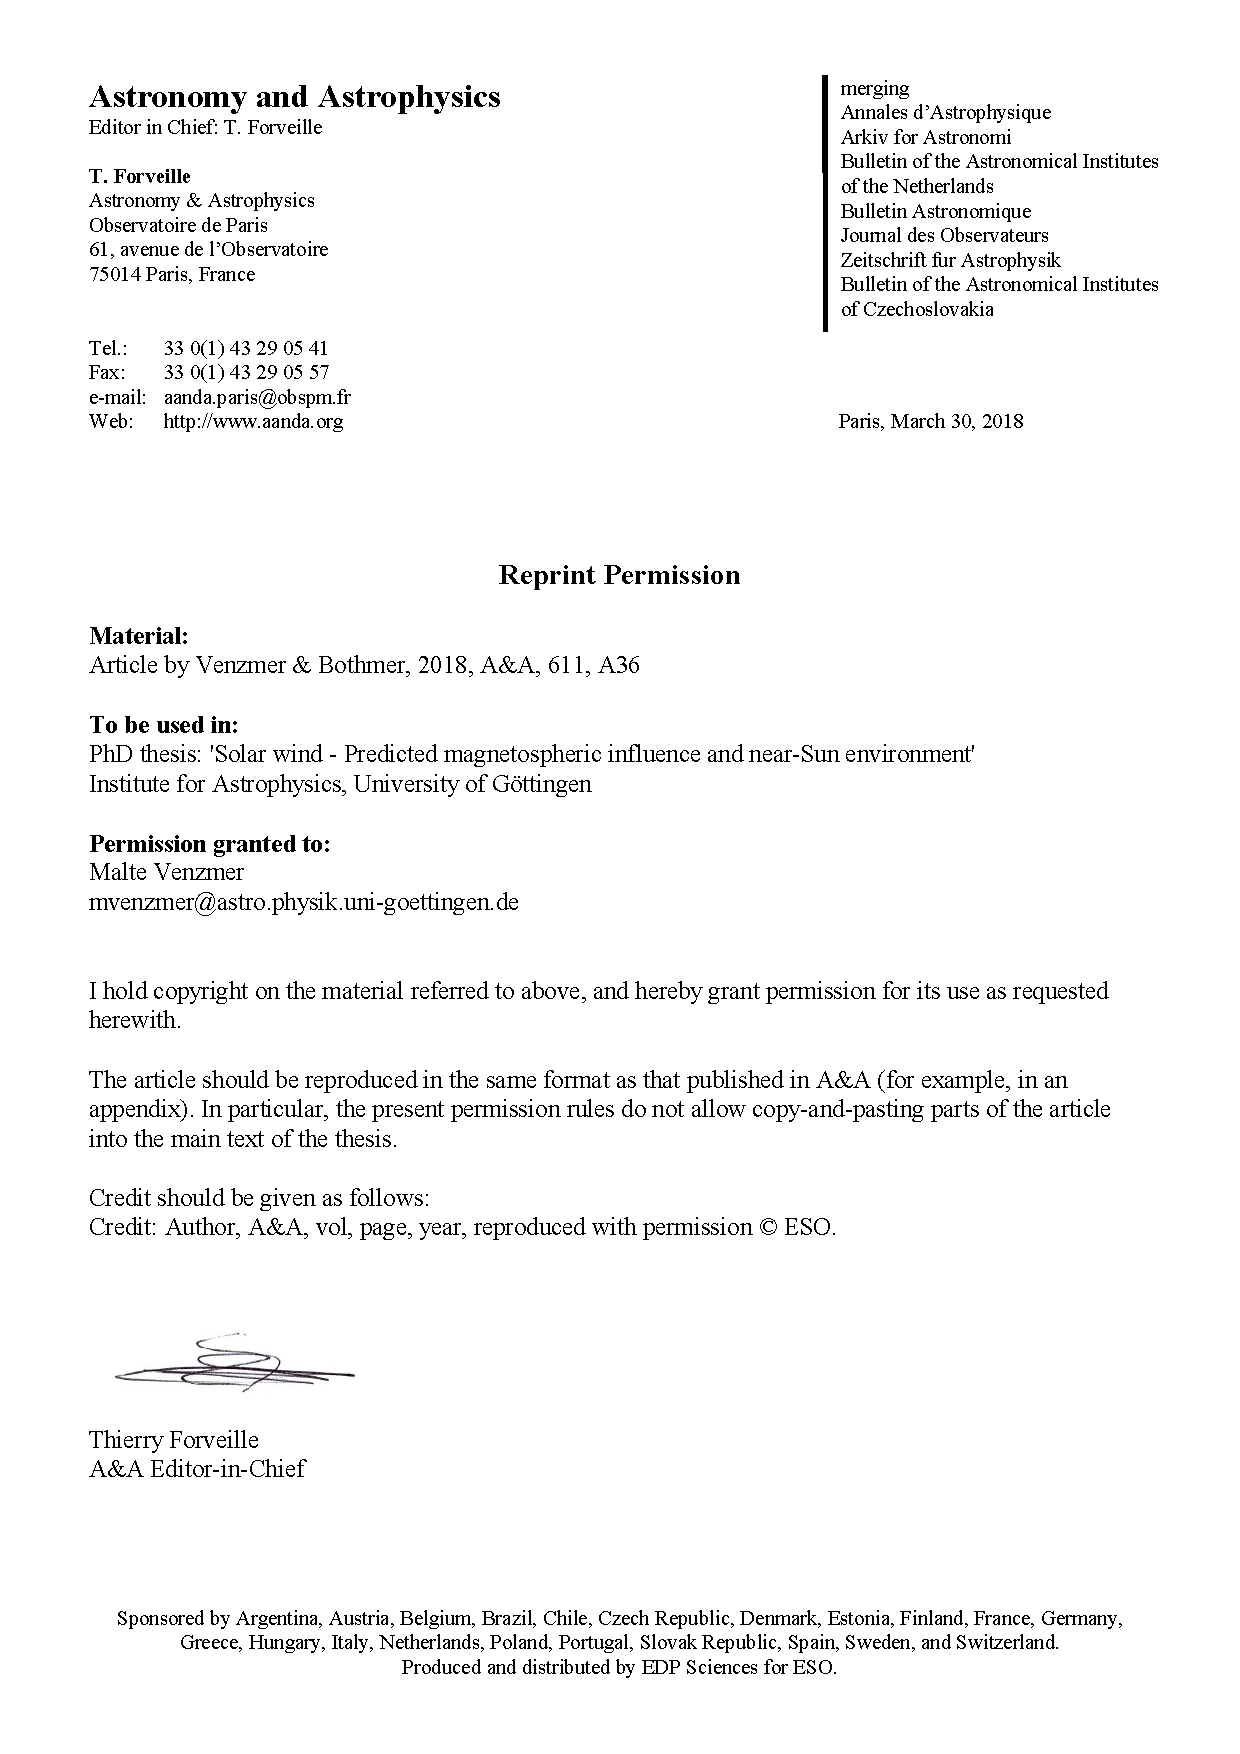
\includepdf[pages={-}]{permissions/c17-046-Venzmer.pdf}


% NASA Media Usage Guidelines:\\
% \url{https://www.nasa.gov/multimedia/guidelines/index.html}
% ``NASA content - images, audio, video, and computer files used in the rendition of 3-dimensional models, such as texture maps and polygon data in any format - generally are not copyrighted. [...] NASA content used in a factual manner that does not imply endorsement may be used without needing explicit permission. NASA should be acknowledged as the source of the material.''\\


\renewcommand\listfigurename{List of figures and their permissions}
\lofimagetrue
\listoffigures



% \begin{itemize*}
% %%% Basics
% 	\item \autoref{fig:sun_interior_HMIIC}: I created the figure from NASA images.
% 	\item \autoref{fig:sun_atmosphere}: I created the figure from NASA images.
% 	\item \autoref{fig:Tse2008_500_mo1}: See the following email correspondence.
% 	\lstinputlisting{figures_of_others/permissions/Druckmuller_permission.txt}
% 	\item \autoref{fig:Owens2013_Heliosphere_screenshot}: See the following RightsLink request result.\\
% 	\fbox{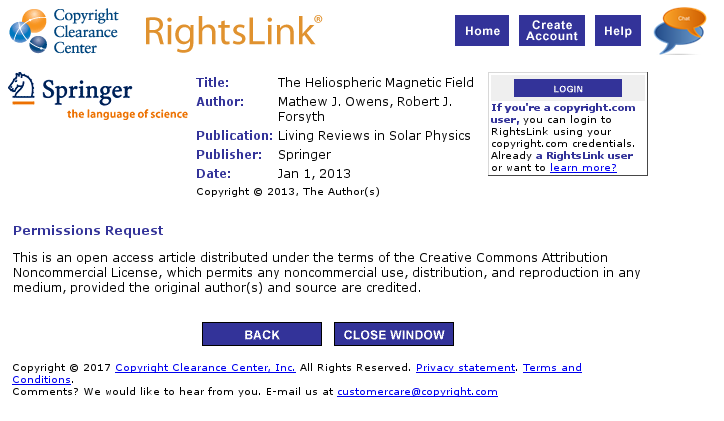
\includegraphics[width=0.7\textwidth]{figures_of_others/permissions/permission_request_Owens2013.png}}
% 	\item \autoref{fig:Miesch2005_fig1a_interior_diff_rot}: See the following RightsLink request result.\\
% 	\fbox{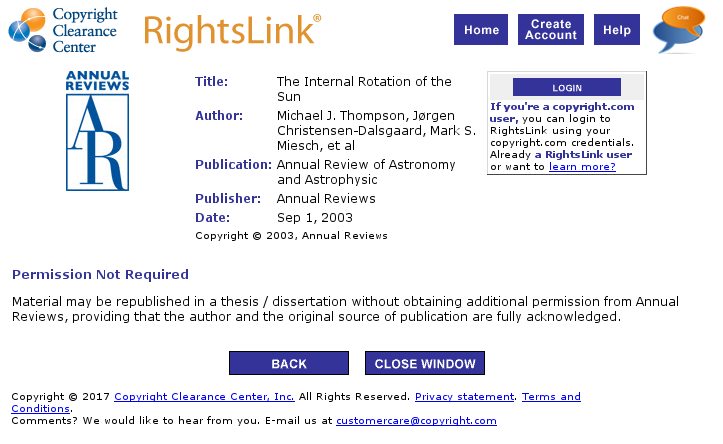
\includegraphics[width=0.7\textwidth]{figures_of_others/permissions/permission_request_Thompson2003.png}}
% 	\item \autoref{fig:Zhao2013_meridional_flow}: See the following email correspondence.
% 	\lstinputlisting{figures_of_others/permissions/Zhao2013_permission.txt}
% 	\item \autoref{fig:bipolar_region_HMIB_HMIIF}: I created the figure from NASA images.
% 	\item \autoref{fig:Hathaway_magbfly}: See the following email correspondence.
% 	\lstinputlisting{figures_of_others/permissions/Hathaway_permission.txt}
% 	\item \autoref{fig:ROB_SSN_wolfmms}: SILSO images can be freely downloaded as public data.\footnote{SIDC/SILSO website, data policy at the bottom: \url{http://sidc.be/silso/home}}
% 	\item \autoref{fig:Cranmer2005_fig1_ab}: See the following email correspondences.
% 	\lstinputlisting{figures_of_others/permissions/Cranmer2005_fig1_IOP_permission.txt}
% 	The related email attachment:
% 	\lstinputlisting{figures_of_others/permissions/Cranmer2005_fig1_permission.txt}
% 	\item \autoref{fig:Banaszkiewicz1998_DQCS_model_raw}: See the following document.\\
% 	\fbox{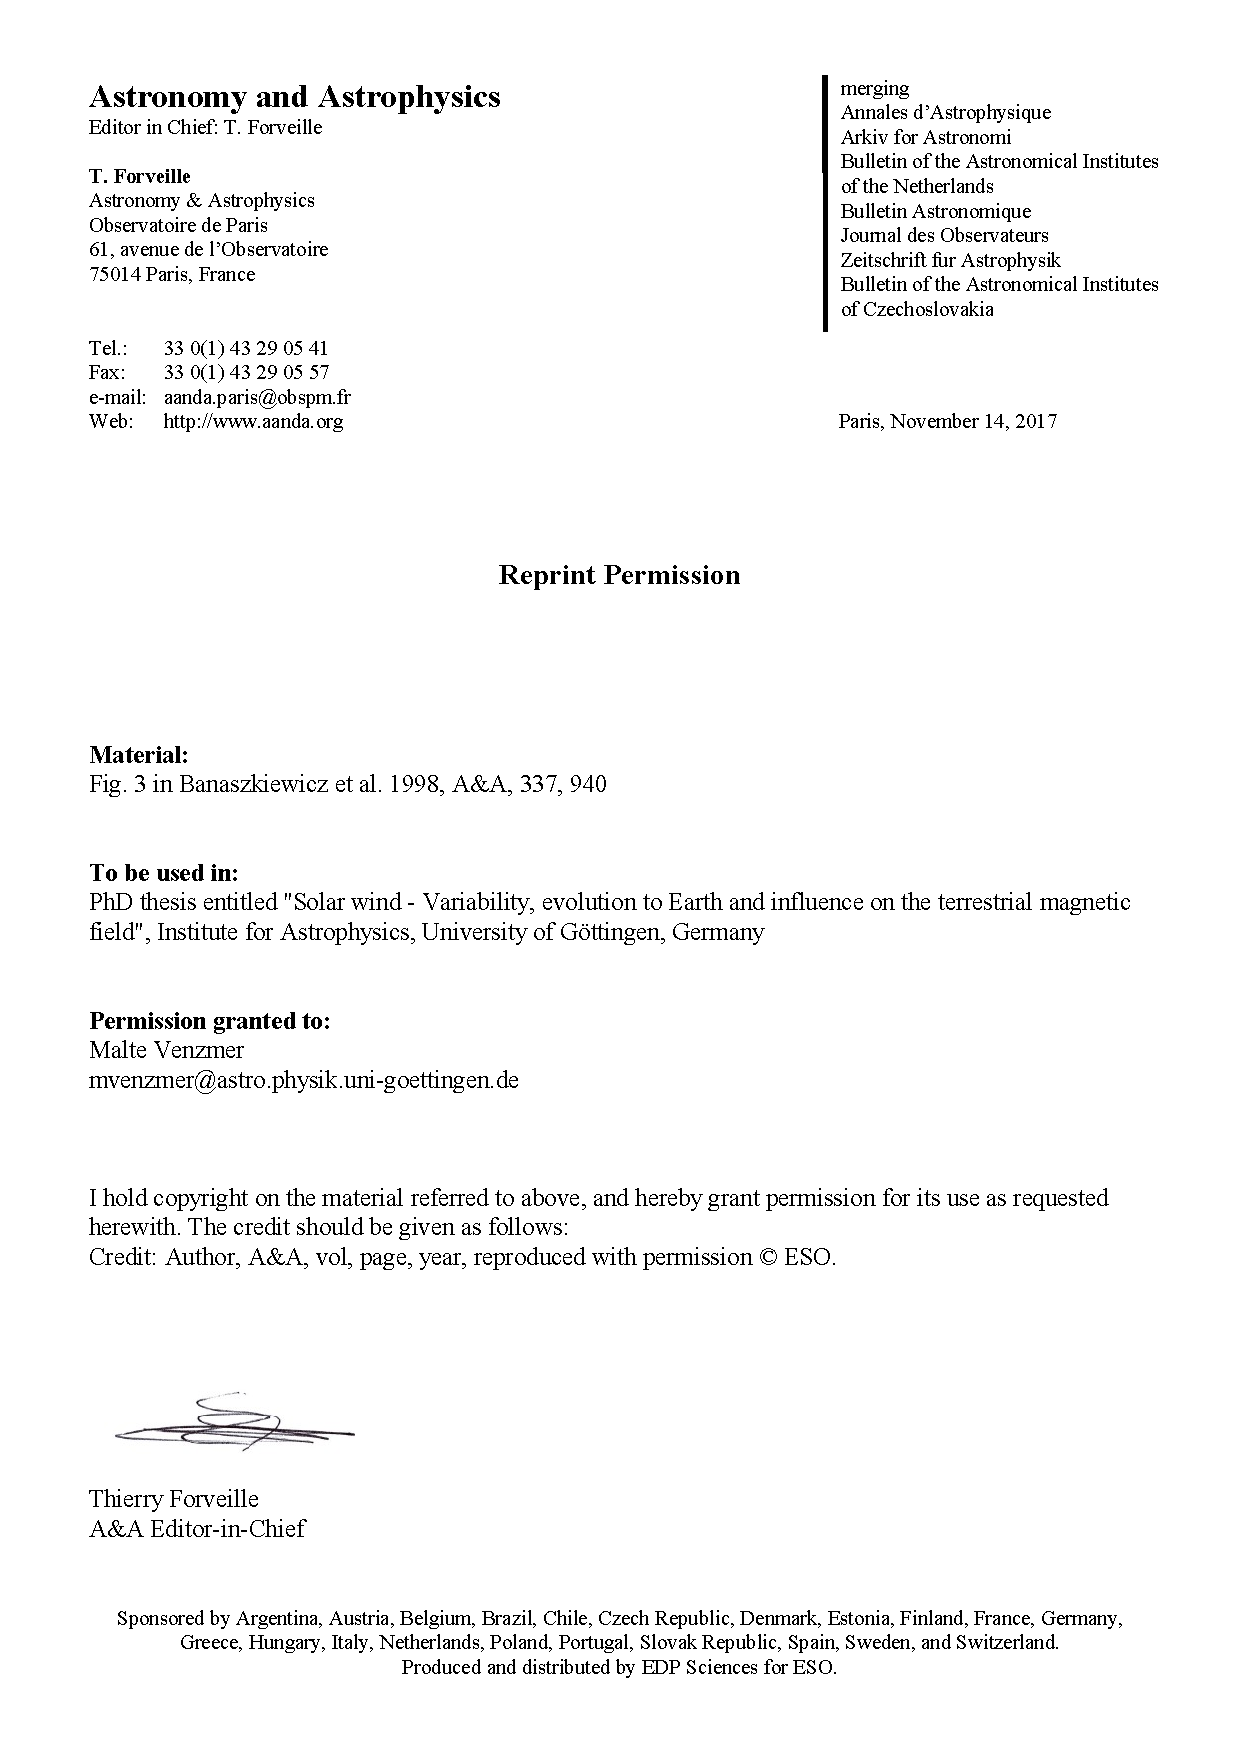
\includegraphics[width=0.6\textwidth,angle=90]{figures_of_others/permissions/permission_request_Banaszkiewicz1998_fig3.pdf}}
% 	\item \autoref{fig:Jokipii1981_ballerina_HCS}: See the following email correspondence.
% 	\lstinputlisting{figures_of_others/permissions/Jokipii1981_permission.txt}
% 	\item \autoref{fig:Owens2013_PFSS_Sectors_screenshot}: See the permission to \autoref{fig:Owens2013_Heliosphere_screenshot}.
% 	\item \autoref{fig:ACE_64s_v7_thesis_CIRs_2013-5-1_65_plot}: I created this figure myself.
% 	\item \autoref{fig:Hundhausen1977_fig10_cut}: ???
% 
% 	\item \autoref{fig:McComas2008_Ulysses_orbit}: See the document on the next page.
% 	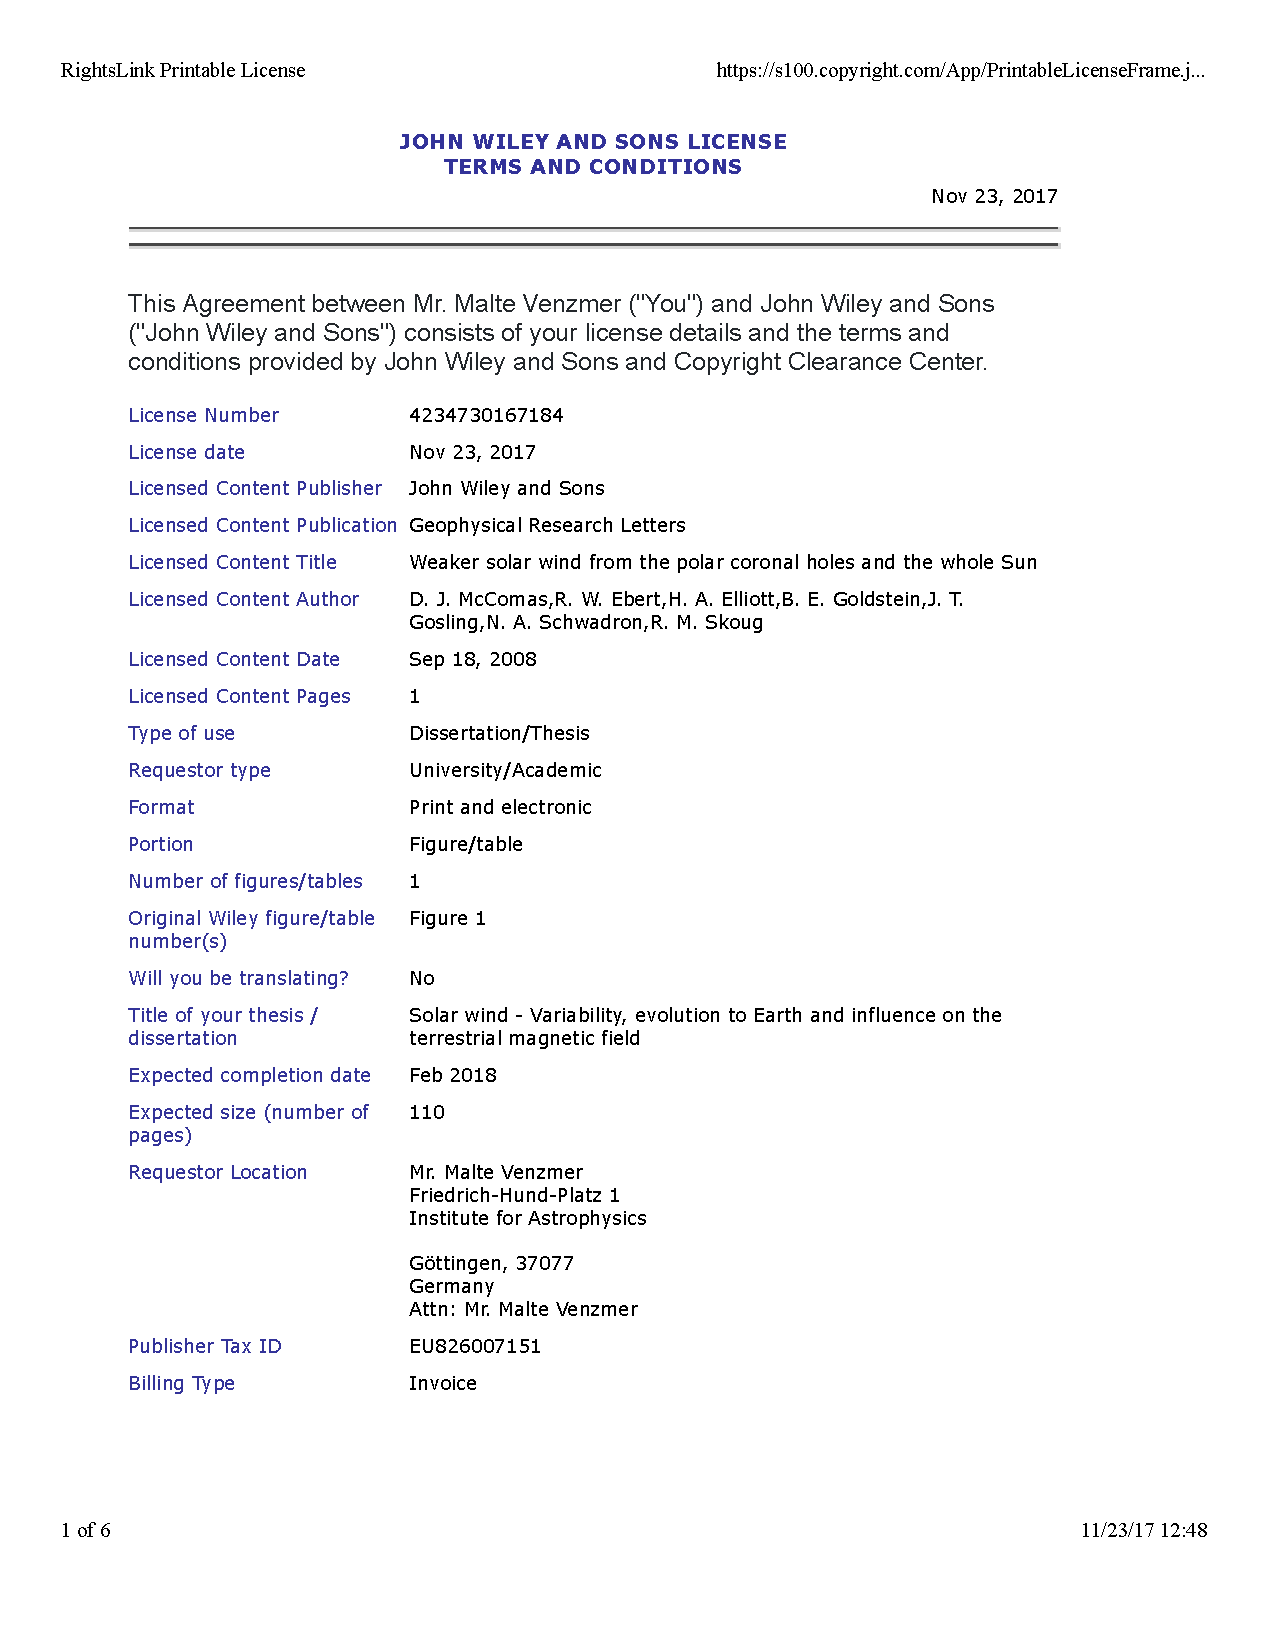
\includepdf[pages={-},nup=2x3,delta=1cm 2mm,column=true,frame=true,noautoscale=true,scale=0.32]{figures_of_others/permissions/permission_request_McComas2008a_fig1.pdf}
% 	\item \autoref{fig:Owens2013_CIR_2panel_screenshot}: See the permission to \autoref{fig:Owens2013_Heliosphere_screenshot}.
% 
% %%% Data
% 	\item \autoref{fig:timeline_SSN_with_data_and_sc}: I created this figure myself.
% 	\item \autoref{fig:ion_energy_spectrum_plot}: I created this figure myself.
% 	\item \autoref{fig:Kp_map}: See the following email correspondence.
% 	\lstinputlisting{figures_of_others/permissions/ISGI_permission.txt}
% 	\item \autoref{fig:musi1612}: The figure is distributed under the Creative Commons license \href{https://creativecommons.org/licenses/by/4.0/}{CC BY 4.0}.
% 	\item \autoref{fig:timeline_OMNI_SC_IDs}: I created this figure myself.
% 	\item \autoref{fig:helios2}: This is a NASA image.
% 	\item \autoref{fig:Helios_r_b_ssn}: I created this figure myself.
% 	\item \autoref{fig:Helios12_orbits_ecliptic_polar}: I created this figure myself.
% 	\item \autoref{fig:helios_data_frequency}: I created this figure myself.
% 
% %%% Chapter2
% 
% 
% 
% 
% %%% Helios-SPP Chapter2
% 	\item \autoref{fig:aa-roll-sc-into-acoustics-cell-0199}: This is a NASA image.
% 	\item \autoref{fig:SPP_ObservingSun2}: This is a NASA image.
% 
% 
% %%% Appendix
% 
% 
% 
% \end{itemize*}





